\documentclass[conference]{IEEEtran}
\usepackage{cite}
\usepackage{amsmath,amssymb,amsfonts}
\usepackage{algorithmic}
\usepackage{graphicx}
\usepackage{textcomp}
\usepackage{hyperref}

\graphicspath{{figs/}}
\begin{document}

\title{Teaching Robots how to Interact with Humans}

\author{\IEEEauthorblockN{Emmanuel Senft}
\IEEEauthorblockA{\textit{Centre for Robotics and Neural Systems} \\
\textit{Plymouth University} \\
Plymouth (UK) \\
emmanuel.senft@plymouth.ac.uk\\
\url{http://www.tech.plym.ac.uk/SoCCE/CRNS/staff/esenft/}}
}

\maketitle

\begin{abstract}

To have meaningful interactiong with humans, robots have to be able to learn,
    and especially learn from humans. My research is focused on how a robot can
    learn how to interact with humans while interacting and being supervised by
    a human teacher.

\end{abstract}

\section{Introduction}

Social interactions are complex environments governs by a large number of social
norms and where any participants have a high number of expections on the others.
As it seems impossible to provide directly a robot with all the knowledge
required to interact with humans, we argue that robots need to be able to learn
how to behave. Furthermore, as the context of interaction and the partners can
evolve over times, robots have to update continuously their behaviours.  The
problem of improving an action policy over time by interacting in an environment
is well represented by Reinforcement Learning. And powerful tools exist to
improve an agent behaviour as it is evolving in an environment, by having a
reward function rating behaviours of the agents, it can improve its behaviour to
maximise the expected behaviour over time and as such reach a better action
policy. 

However classic method in Reinforcement Learning are relying on exploration,
often random to acquire information on the environment and often require many
iterations to converge to an appropriate action policy. When interacting with
humans in the real world, acquiring data can take a prohibitive time, and the
risk of exploration can be high: failing to validate expectations from human
partners can lead to stopping the interaction or even annoy partners. To tackle
this issue, we propose to make use of a human supervisor to guide the robot
behaviour, preventing it to make mistakes and demonstrating it a correct action
policy.

\section{Proposition}

\subsection{Supervised Autonomy}

Robot cannot have optimal behaviours, especially in the early stages of
learning. The idea behind Supervised Autonomy is to have a robot mostly
autonomous, but supervised by a human. Before executing an actions, the robot
proposes this action to a supervisor who is able to correct it before execution,
ensuring that only actions validated by a human are executed. 

This validation of action is combined with an automatic execution after a short
delay: for all correct actions, the supervisor does not have to interact and can
let the robot being autonomous, only in cases where the proposed actions is
incorrect, the supervisor has to step in.

traditional approach use humans as label, to provide feedback on actions
executed by the robot. I aim to give more power to the teacher to let them stear
the robot behaviour in the desired direction.


\subsection{SPARC}

When the robot is interacting in a Supervised Autonomous fashion, it can also
use the human inputs to improve its behaviour over time. Combined with
algorithms from the Reinforcement Learning field, this approach can ensure that
the behaviour of the robot is constantly correct, and the frequency of
intervention from the supervisor decreases.

Other methods using humans to teach a robot how to interact often use the human
only to label actions from the robot, to provide corrective behaviours once
the robot has made a mistake or have the robot request a demonstration from the
human when its confidence in the output of the learning algorithm is too low.
SPARC is the only method giving total power to the human on the robot behaviour
without requesting him to manually enforce every actions.
Figure~\ref{fig:comparison} show an illustrative comparison between SPARC and
other learning methods. By giving control on \emph{every} robot's action to the
teacher, SPARC is the only method allowing the robot to have an efficient
behaviour even in early stages of the learning.

\begin{figure}
    \centering
    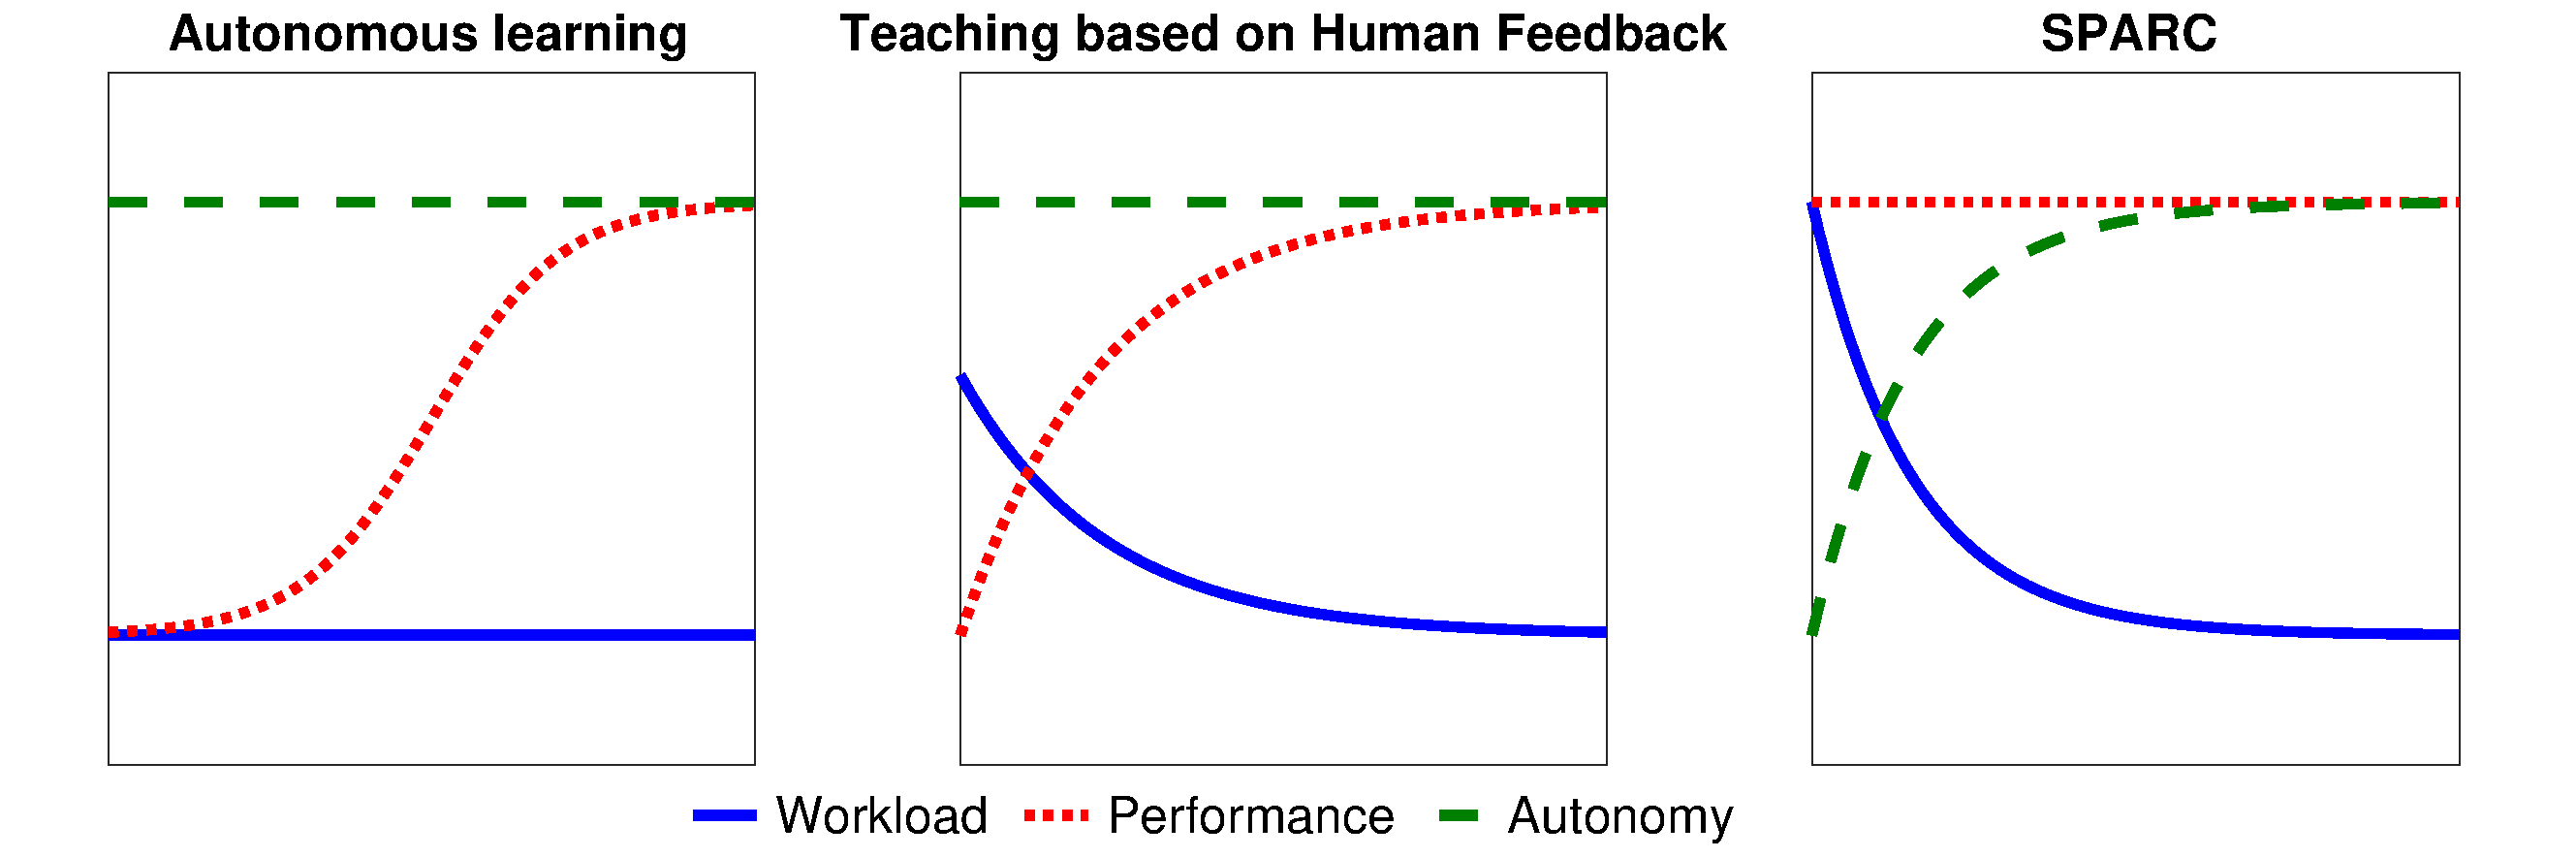
\includegraphics[width=0.9\linewidth]{motivation.pdf}
    \caption{Comparison of workload on human teacher, performance of the robot
    and autonomy for three frameworks of learning: autonomous learning, learning
    with human feedbacks and SPARC}
    \label{fig:comparison}
\end{figure}

\section{Experiments}

SPARC has been tested in two explorative studies and so far has demonstrated
promising results.

\subsection{Initial Eploration with Direct Mapping}
ICSR
\subsection{Combining Supervised Autonomy with Reinforcement Learning}
Sophie's Kitchen

\section{Discussion}

\section{Future work}

\section*{Selected publication}
\begin{itemize}
        \item E. Senft, P. Baxter, J. Kennedy, and T. Belpaeme, “Sparc:
            Supervised progressively autonomous robot competencies,” in
            International Conference on Social Robotics, 2015, pp. 603–612.
            %\cite{senft2015sparc}
        \item E. Senft, P. Baxter, J. Kennedy, S. Lemaignan, and T. Belpaeme,
            “Supevised autonomy for online learning in human-robot interaction,”
            Pattern Recognition Letters, 2017. %\cite{senft2017supervised}
\end{itemize}


%\bibliographystyle{IEEEtran} \bibliography{biblio}

\end{document}
